\documentclass[11pt]{article}
\usepackage[french]{babel}
\usepackage[T1]{fontenc}
\usepackage{fontspec}
\usepackage[utf8]{inputenc}
\usepackage{url}
\usepackage{eurosym}
\usepackage{pdfpages}
\usepackage{ulem} % to use a strikeout/strikethrough font
\usepackage{color}
\newcommand{\fs}[1]{\textcolor{red}{\sout{#1}}}
\newcommand{\f}[1]{\textcolor{blue}{#1}}
\usepackage{graphicx} % Inclure des images
\usepackage{multicol} % Multi-colonnes


\usepackage[autolanguage, np]{numprint} % écriture des virgules
\usepackage[top=3cm,right=2cm,bottom=2cm,left=2cm]{geometry}

\title{HAUM}
\author{Assemblées Générales Ordinaire \& Extraordinaire}
\date{17 Novembre 2015}

\begin{document}
\maketitle


\section*{Convocation}

Madame, Monsieur,

L'association HAUM vous convoque à ses Assemblées Générales Ordinaire \& Extraordinaire qui se tiendront le :

\begin{center}
{\Large 10 Novembre 2016 à 19h00}\\
à la Ruche Numérique,\\19 Bd M\&A Oyon au 1\textsuperscript{er} étage,\\72 100 Le Mans
\end{center}

En cas d'impossibilité, veillez vous faire excuser et vous faire représenter si vous le souhaitez (2 procurations maximum par personne présente, Statuts, art. 6).

\vspace{1.5cm}

\hrule
\vspace{.3cm}
\begin{center}
\Large\bfseries Assemblée Générale Extraordinaire
\end{center}
\vspace{.3cm}
\hrule

\vspace{1.5cm}

\section*{Déroulement}

\begin{enumerate}
    \item Appel et annonce des procurations
    \item Amendement aux statuts sur la vente de biens (porté par le bureau)
    \begin{itemize}
        \item Exposé
        \item Débat
        \item Vote
    \end{itemize}
\end{enumerate}


\section{Amendement aux statuts sur la vente de biens}

L'amendement est porté par le bureau.

\subsection{Exposé}

Durant l'année passée, le HAUM a été amené à vendre des biens lui appartenant, soit des éléments d'objets démontés (vendus pour pièces) ou plus récemment des produits de l'activité (Laumios). Cette vente n'est légale qu'à la condition que les statuts reflètent cette activité. Cette amendement vise à mettre l'association en conformité avec la loi.

Il est proposé l'ajout d'un article après l'article 4 intitulé ``Ressources'' ainsi rédigé :

\begin{quotation}
\itshape
\noindent Les ressources de l'association sont constituées de :
\begin{itemize}
    \item cotisations 
    \item dons ou legs
    \item vente ou location de biens appartenant à ou produits par l'association
\end{itemize}
Ces ressources peuvent être utilisées à toutes fins utiles comprenant notamment mais pas exclusivement l'achat de matériel, le financement de projets, la publicité ou le transport pour des évènements.
\end{quotation}

\subsection{Débat}
\subsection{Vote}

\section*{Clotûre}

\vspace{1.5cm}

\hrule
\vspace{.6cm}
\begin{center}
\Large\bfseries Assemblée Générale Ordinaire
\end{center}
\vspace{.3cm}
\hrule

\vspace{1.5cm}

\section*{Déroulement}

\begin{enumerate}
    \item Présentation de l'association
    \item Rapport moral
        \begin{enumerate}
            \item Bilan
            \item Objectifs
            \item Questions
        \end{enumerate}
    \item Rapport financier
        \begin{enumerate}
            \item Bilan \& Objectifs
            \item Previsionnel 2017
            \item Questions
        \end{enumerate}
    \item Motions et vote
    \item Election du nouveau bureau
    \item Questions diverses
\end{enumerate}

\section{Présentation de l'association}

% TODO

\section{Rapport Moral}

\subsection{Bilan}

Cette année a été riche en changements et en actions menées pour et par l'association.

\subsubsection{Changement de local}

Après près de 2 ans dans nos anciens locaux au sein de la pépinière de la Ruche Numérique, le HAUM commençait à se sentir à l'étroit. Pour que les séances se déroulent dans les meilleures conditions de confort et de sécurité, il était temps de changer de local.

Cette envie a pu se concrétiser grâce au concours de Le Mans Développement, agence de développement économique de la métropole, qui a mis a notre disposition un local 2 fois et demi plus grand (passant donc de 29m\textsuperscript{2} à plus de 70m\textsuperscript{2}). Le Mans Développement a également réalisé les travaux nécessaires à l'installation de l'association et nous a mis en relation avec les services techniques de la ville du Mans pour que nous puissions récupérer du mobilier mis au rebut et ainsi meubler le lieu.

L'établi du HAUM est toujours mis à sa disposition par la Ruche Numérique malgré notre départ de leurs locaux.

Le bureau tient à remercier tous les acteurs institutionnels et les bénévoles qui ont rendu possible ce déménagement.

\subsubsection{Évolution des adhésions}

Au cours de l'année 2016, le nombre d'adhésions est passé de 35 à 41.
Il est à noter qu'environ 25 membres de l'année précédente n'ont pas renouvelé leur adhésion. L'association a par conséquent connu un changement massif de sa base de membres.

\subsubsection{Participation au projet French Tech}

Les discussions pour le changement de local font partie d'un projet plus vaste de création d'un pôle d'activité sur le secteur de la Gare dans le cadre du label French Tech. L'objectif est de mettre en oeuvre une Cité de l'Innovation Colaborative (CICO) rassemblant un certain nombre d'acteurs. L'inclusion du HAUM dans le projet (en tout cas sa présence sur le lieu de l'éventuelle CICO) a permis au Mans d'obtenir le label French Tech.

Dans le cadre de ce projet, les discussions portent à la fois sur la réhabilitation de l'ancien hôpital spécialisé de la rue Étoc Demazy mais également sur une "première phase" à plus court terme qui prendrait place dans les locaux de l'ancienne DDCS (Boulevard Lefaucheux). Cet aménagement permettrait de rassembler un incubateur, une pépinière et le hackerspace dans 1000m\textsuperscript{2}.

L'implication principale porte sur le déménagement du HAUM à court ou moyen terme. Il va donc être nécessaire de planifier ce déménagement, afin de minimiser les éventuels problèmes lors de celui-ci.

Cette planification ne peut se faire qu'avec le concours des partenaires institutionnels qui tendent à partager difficilement les informations. Affaire à suivre.

\subsubsection{Animations publiques}

Comme à l'accoutumée, le HAUM a contribué \& organisé en 2016, plusieurs animations à destination du public.

\paragraph{24H du code} Pour l'édition 2016 des 24H du Code (co-organisées par l'ENSIM et la Ruche Numérique), le HAUM a proposé un sujet. Le sujet portait sur la création d'un outil pour explorer des données fournies par Sarthe Développement (ouverture des lieux touristiques). Plusieurs membres du HAUM ont ainsi collaborer pour rédiger le sujet mais aussi être présent toute la nuit aux 24h du code pour guider les équipes.

\paragraph{Bienvenus sur Mars} Organisé au prieuré de Vivoin, le festival BienVenus sur Mars a invité le HAUM a présenter son Pong1D, le dHAUM mais également une création originale. Les Laumios sont nés ainsi et ont engendré de nombreuses idées de projets futurs. La vente de Laumios n'est pas exclue et l'affaire est à suivre.

\paragraph{Gamers Assembly} La Gamers Assembly accueille depuis 2 ans un village \textit{maker}. Cette année, l'organisation a convié le HAUM pour y présenter quelques réalisations. Ce fut l'occasion pour certains de nos membres d'aller pour la première fois sur une aussi grosse manifestation.

\paragraph{Siestes Teriaki} Après les siestes il y a deux ans et le festival l'an dernier, le HAUM est revenu à Teriaki cette année avec le projet Lampes Orbitales (également présenté à Vivoin), un mini-spectacles sur Laumios et un labyrinthe géant. L'organisation de l'évènement a posé de nombreux problèmes de gestion du temps et la question se pose désormais : doit on continuer à prendre part à des manifestations demandant autant de travail ?

\paragraph{Le sHAUM} Suite à son déménagement, le hackerspace a invité ses partenaires à venir découvrir le nouveau lieu. Ce fut une bonne occasion pour discuter avec toutes et tous et de faire découvrir l'association et ses possibilités.

\paragraph{Les HAUMTalks} L'association a organisé 6 sessions de ses mini-conférences en 2016 et au moins une septième est prévue. Les HAUMTalks intéressent un public assez large et permettent à chacun de présenter des sujets lui tenant à coeur (hacker). Ces rencontres permettent aussi de faire connaître l'association auprès d'extérieurs.

\subsubsection{Partenariats et Réseau}

Dans le cadre des différentes manifestations auxquelles il a participé et des différents projets auxquels il prend part, le HAUM continue de développer un réseau d'acteurs et de partenaires proches. Parmi eux : Teriaki, le Hangar Créalab, la compagnie Organic Orchestra, le CESI, la Ruche Numérique, l'ENSIM, la CCI du Mans et de la Sarthe, Le Mans Développement, Sarthe Développement, Le Mans Métropole, etc...

Merci à eux.

Le HAUM a pu participer à la Gamers Assembly 2016 grâce à l'association Rurart. L'association tient également à remercier QuaiLab, Les Usines Nouvelles et les petits débrouillards Poitou-Charente pour leur accueil et les échanges durant l'évènement.

\subsubsection{Projets}

Parmi les très nombreux travaux menés en séance, nous retiendrons tout particulièrement :

\begin{itemize}
    \item Lampes orbitales/Laumios
    \item LaumioAnimator
    \item Labyrinthe Initiati
    \item Améliorations de la fraiseuse
    \item Stations de soudage
    \item sHAUM
    \item Amélioration du 1DPong (lors de la Gamer's Assembly)
    \item Reconstruction du PianoStairs
\end{itemize}

Ces différents projet permettent de faire vivre et connaître l'association. Merci à tous ceux qui y ont pris part en les construisant, en les documentant, en les \textit{hackant} et en les faisant évoluer.

\subsubsection{Communication}

Depuis sa création officielle en 2012, le HAUM souffre de problèmes chroniques de communication. En effet, qu'elle soit à destination des membres ou des extérieurs, la communication du HAUM reste spécifique et non-inclusive.

À toutes fins utiles, le bureau tient à rappeler que le moyen de communication officiel de l'association est la liste de discussion par mail.

Les problèmes de communication ont notamment conduits à des malentendus avec nos partenaires, des retards dans la propagation de l'information et des soucis d'organisation plus larges. À l'échelle du hackerspace, la communication trop sporadique entre les membres a privé certains d'opportunités intéressantes et mené d'autres à s'écarter de l'association ou en tout cas des rôles qu'ils y occupaient.

À un autre égard, le manque de réponse sur l'adresse contact cause de graves lenteurs dans nos rapports aux autres et renvoie une image très statique du HAUM.

À l'avenir, il pourrait être intéressant de désigner 2 personnes responsables de \texttt{contact@haum.org} (tout en étendant la diffusion pour information au bureau) de même qu'il est nécessaire d'améliorer rapidement la communication des informations au sein de l'association. Les personnes en charge des relations avec les partenaires extérieurs \textbf{doivent} s'acquitter du transfert de l'information vers la mailing-liste (et pas uniquement en séance). Les informations importante, même confidentielles, doivent également être transférées \textit{a minima} sur la liste du bureau, sinon évoquées en réunion de bureau.

La vie du hackerspace est une affaire commune, ses relations vers l'extérieur également.

\subsection{Objectifs}

L'année 2016 a vu naître et progresser bon nombre de partenariats et de discussion. Il est donc raisonnable d'espérer que 2017 apportera son lot de nouveau matériel et de nouvelles relations.

Il est temps également de travailler sur l'axe de mutualisation des moyens pour que chacun des membres puisse réaliser ses envies et qu'un minimum d'argent soit perdu en doublons.

Le déménagement a entrainé la perte de l'accès à Internet et il est également nécessaire de remédier à cela dans les mois à venir pour garantir à tous un accès convenable aux ressources.

Les prestations et actions extérieures sont bien sûr à poursuivre et à encourager. Il faudra par ailleurs simplifier les relations avec les partenaires afin d'éviter les malentendus encore trop courants. La réalisation de prestations contribue au financement de l'association et il est souhaitable qu'un maximum de membres y participent.

Enfin, parce que l'association compte toujours plus de membres, il faudra travailler à l'amélioration des locaux pour permettre de l'utiliser comme lieu de travail bien sûr mais également comme lieu de vie et d'échange. Le HAUM vise à proposer une vision alternative du rapport à la technologie et si cela passe bien sûr par les aspects techniques, cela peut également être renforcé par des temps d'échanges informels (Jeudi du Libre) ou non (HAUMTalks).

\section{Rapport financier}

\subsection{En images}
Nous présentons ici un focus des comptes à la date d'aujourd'hui. Le bilan financier 
sera présenté au début de l'année 2017 par mail. Cela permettra d'établir les comptes 
au 31 décembre.
\begin{center}
\begin{multicols}{2}
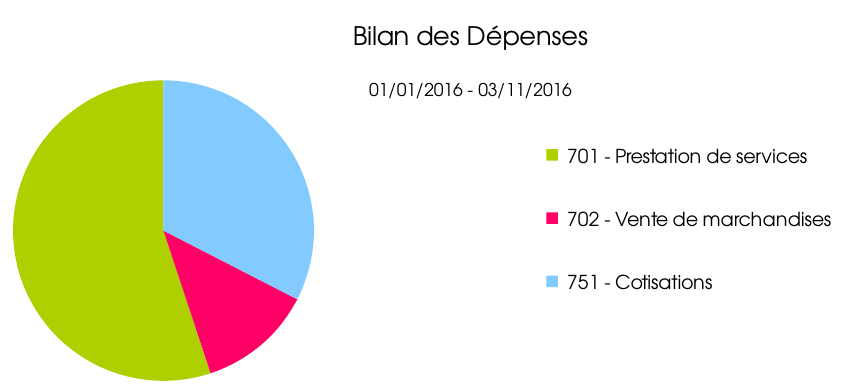
\includegraphics[width=8cm]{1DossierAGRecettes.png}

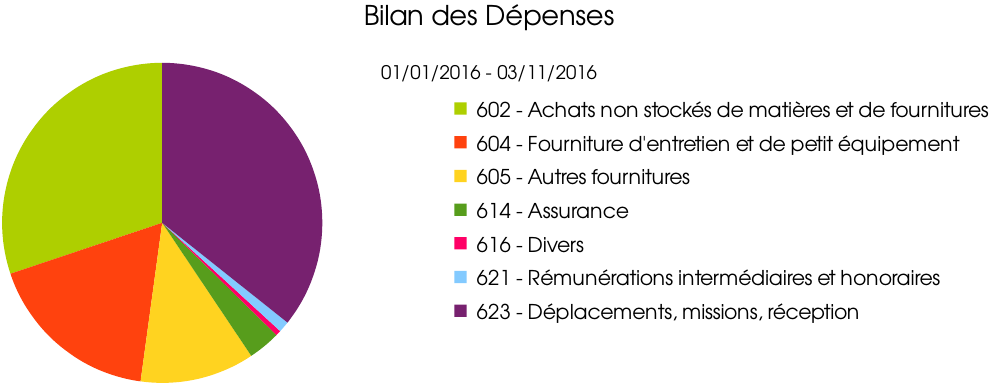
\includegraphics[width=8cm]{2DossierAGDepenses.png}
\end{multicols}

\begin{multicols}{2}
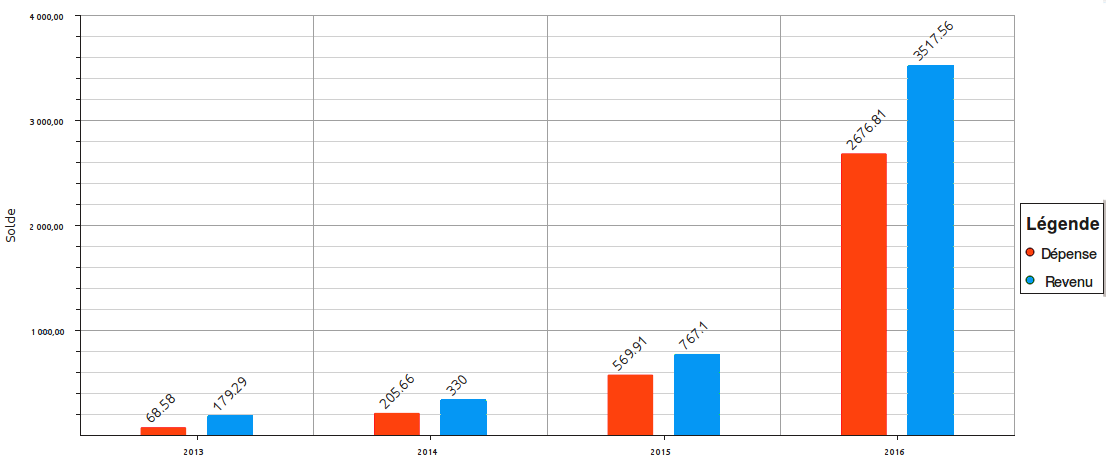
\includegraphics[width=8cm]{3DossierAGGeneral.png}

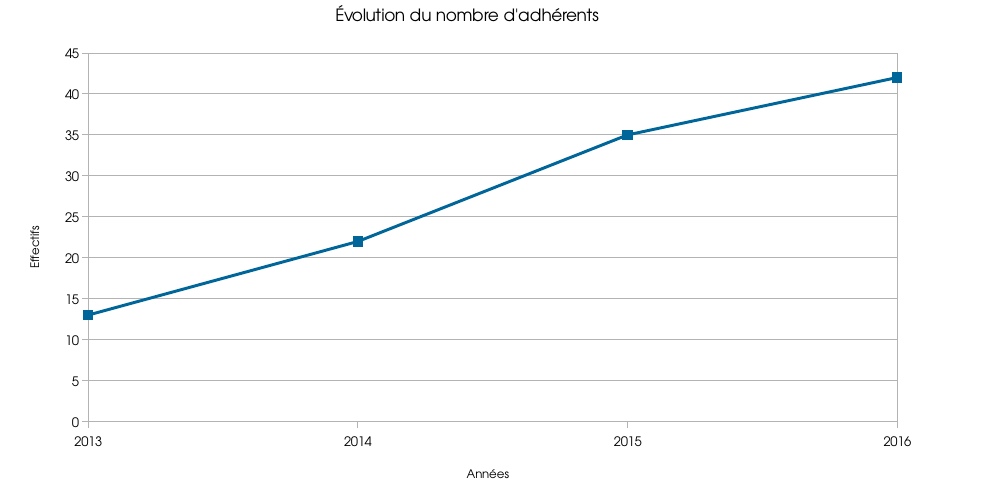
\includegraphics[width=8cm]{4DossierAGAdherents.png}
\end{multicols}
\end{center}
\subsection{Bilan et objectifs}
L'ensemble des comptes de l'association depuis sa création a été repris de manière 
à obtenir une tenue de comptes exacte et conforme au Plan Comptable Général français.

Nous pouvons alors remarqué que les volumes financiers sont en forte croissance 
cette année.

L'année dernière nous avions pour objectif la mutualisation des moyens matériel. 
On progresse bien dans cette voie : il nous a été possible d'acheter une perceuse à 
colonne, un \textit{plotter} de découpe et un jeu de tournevis.
Il est maintenant possible de gérer le consommable sans difficulté et d'assumer dans
une moindre mesure le besoin en trésorerie pour la réalisation des projets pour lesquels 
une rétribution nous est donnée.

Si on souhaite être en capacité de financer des machines ou de l'outillage plus onéreux 
ou en plus grand nombre, l'augmentation des cotisations, des mécénats et/ou des 
actions qui seraient capables de nous rapporter de l'argent serait la bienvenue.

\bigskip

Cette année encore des difficultés de gestion de trésorerie ont été rencontrées. Ce qui 
nous amène à réaffirmer les règles instaurées l'an passé : 
\begin{itemize}
 \item Toutes les factures doivent être établies \textbf{au nom du HAUM} et ne 
 contenir que des éléments \textbf{achetés pour le HAUM}. 
 \item Les dépenses de l'argent du hackerspace ne doivent être faites qu'après 
 \textbf{consultation des autres membres} et, surtout, \textbf{vérification de la 
 trésorerie}.
\end{itemize}
De plus, les dépenses augmentant significativement, avant toute dépense d'argent, une 
demande de validation \textbf{par mail} devra désormais être effectuée.

Le focus financier contient, à ce jour, un impayé de 250\euro concernant un chèque refusé 
à trois reprises. Des démarches sont actuellement en cours pour y remédier.

\subsection{Prévisions 2017}

Pour l'année à venir, le budget prévisionnel a été construit sur la base des charges 
et des recettes de l'année 2016.

\subparagraph{Recettes}
Il est estimé pour les recettes :
\begin{itemize}
 \item 437,31~\officialeuro{} de prestations ;
 \item 170~\officialeuro{} de vente de marchandises ;
 \item \np{1377,60}~\officialeuro{} de cotisations ;
 \item \np{8966}~\officialeuro{} de subvention exceptionnelle pour l'achat d'une découpeuse laser.
\end{itemize}

\subparagraph{Charges}
Pour les charges, il est prévu :
\begin{itemize}
 \item 260~\officialeuro{} pour l'achat de fournitures ;
 \item 508,03~\officialeuro{} pour les petits équipements ;
 \item 246~\officialeuro{} pour les autres fournitures (par exemple, en 2016, les tee-shirts) ;
 \item 150~\officialeuro{} pour la communication (cartes de visites, ...) ;
 \item 450~\officialeuro{} pour les frais de déplacement, de réception, ... ;
 \item 239,88~\officialeuro{} pour une connection internet indépendante ;
 \item \np{8966}~\officialeuro{} achat de la découpeuse laser.
\end{itemize}

\subparagraph{Bénévolat}La valorisation du bénévolat sera établie régulièrement lors des réunions mensuelles. 
Elle a été estimée à \np{8142}~\officialeuro{} pour l'année prochaine.

\subparagraph{}Le budget prévisionnel est alors de \np{28392,91}~\officialeuro{}.

\section{Motions}
Aucun amendement au Règlement Intérieur n'a été proposé.

\section{Questions Diverses}

\newpage

\clearpage
\thispagestyle{empty}
\topskip0pt
\vspace*{\fill}
\begin{center}
\hrule
\vspace{.3cm}
\Huge\bfseries Annexes
\vspace{.3cm}
\hrule
\vspace{2cm}
\Large
\noindent Bilan Financier 2016\\
Bilan Général 2013-2016\\
Budget Prévisionnel 2017
\end{center}
\vspace*{\fill}

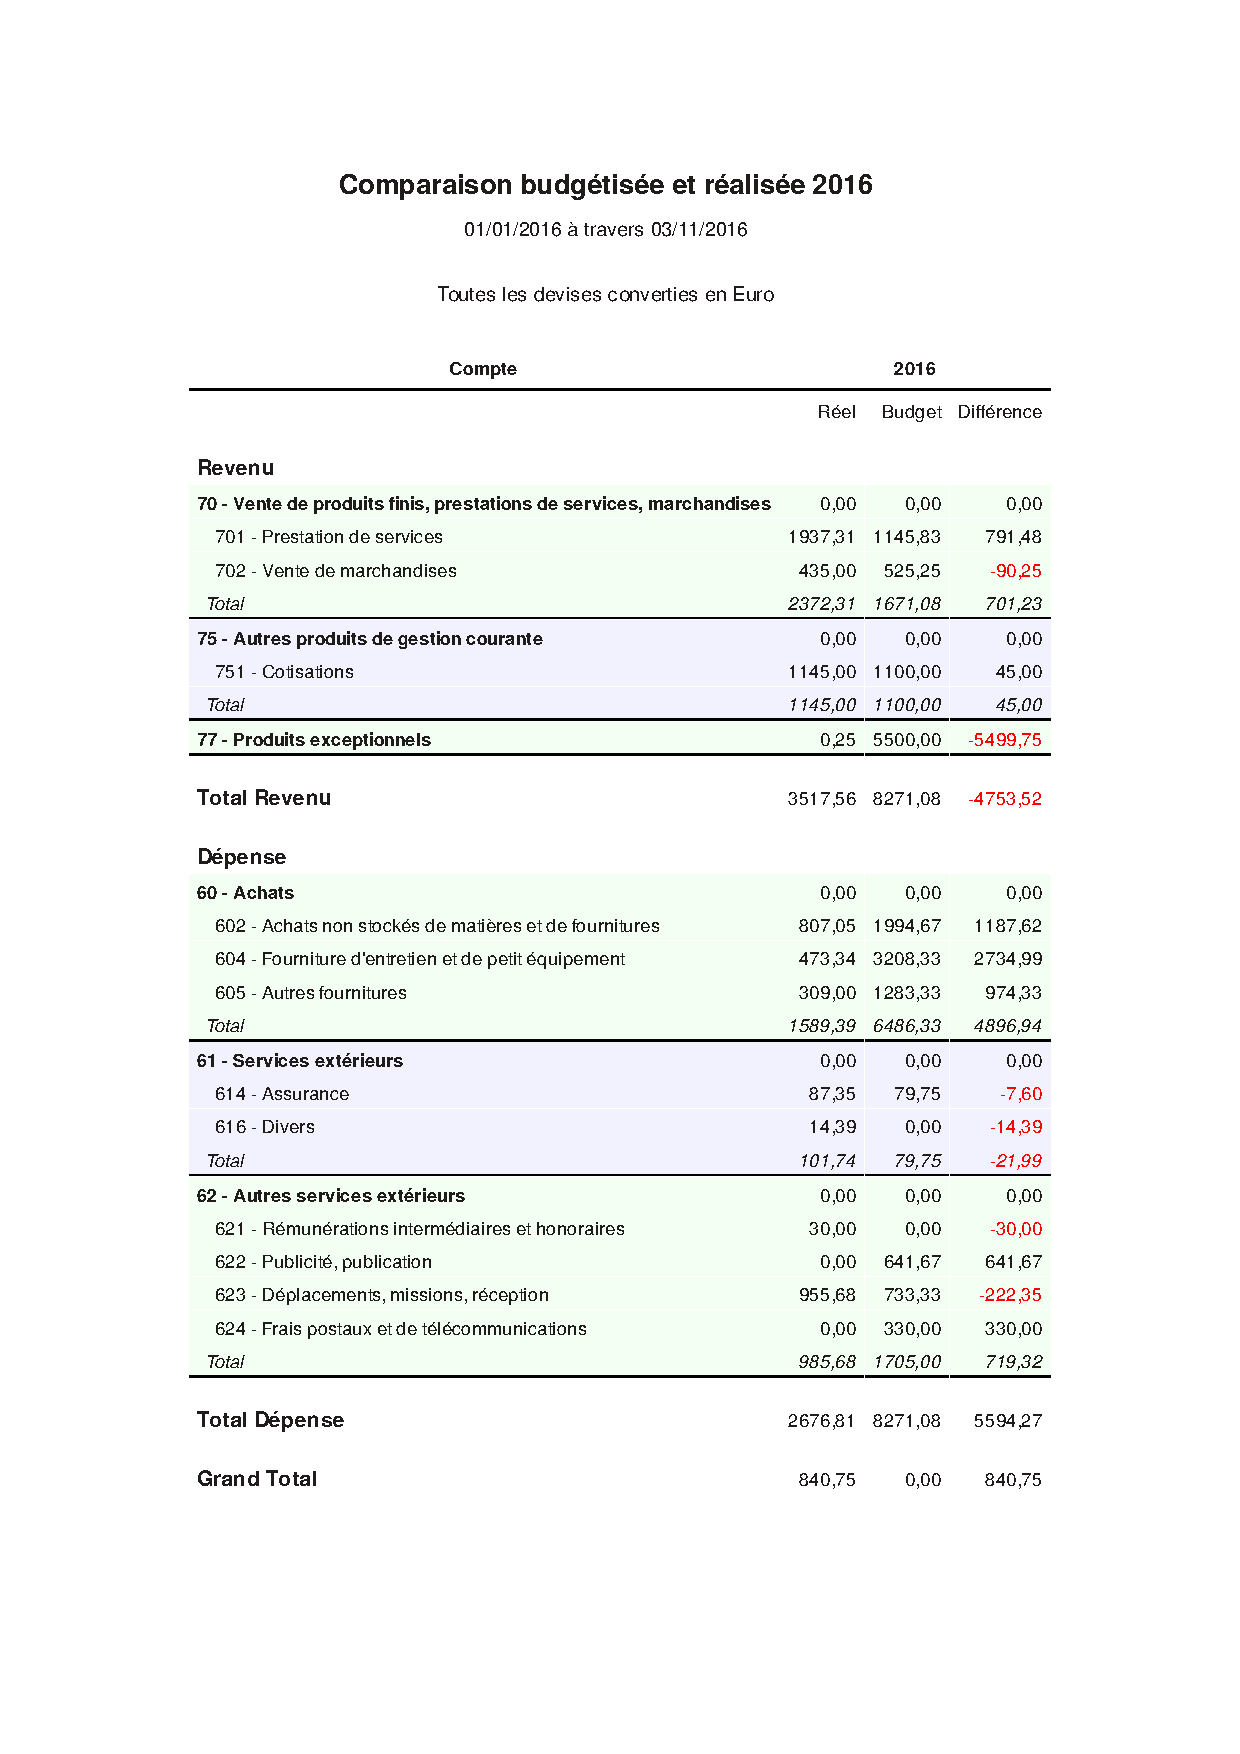
\includepdf[pages=-]{BilanFinancier2016.pdf}
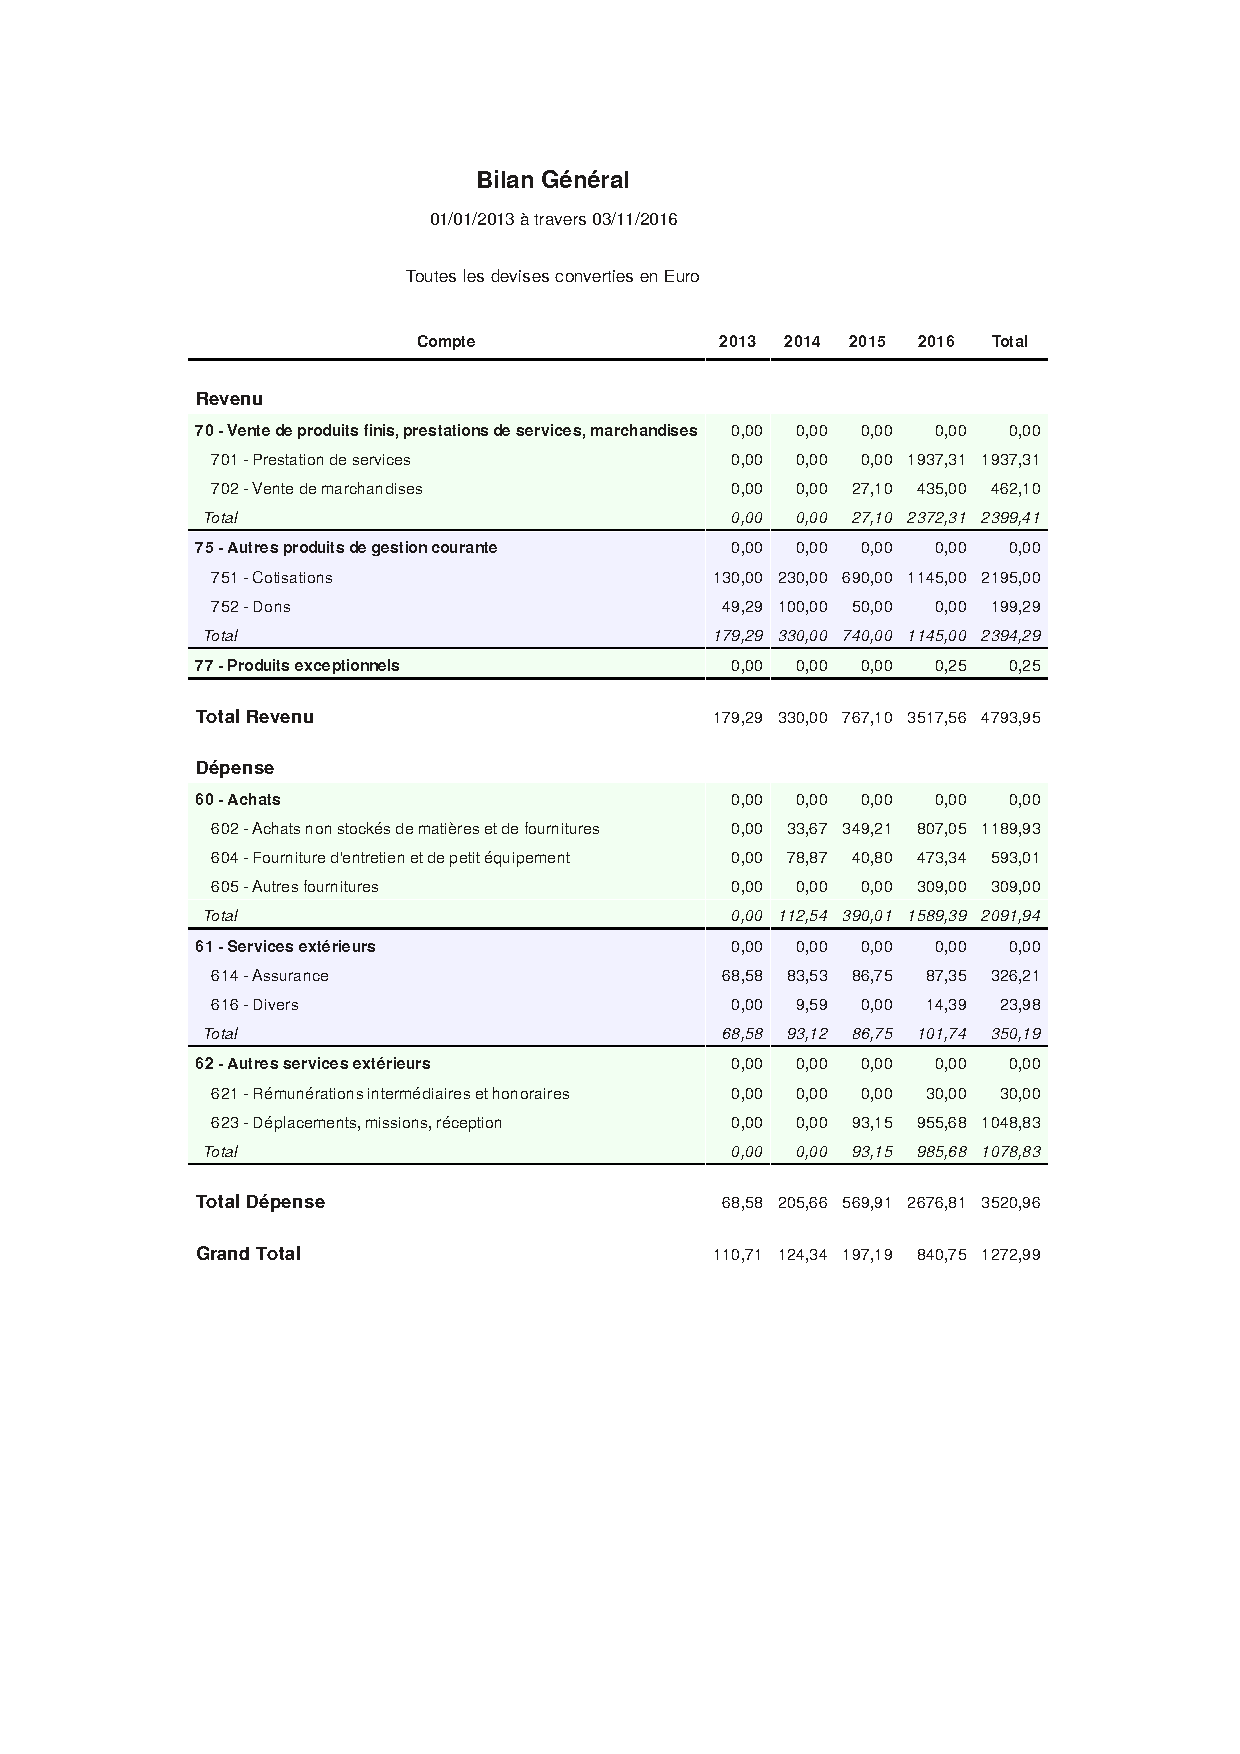
\includepdf[pages=-]{BilanGeneral2016.pdf}
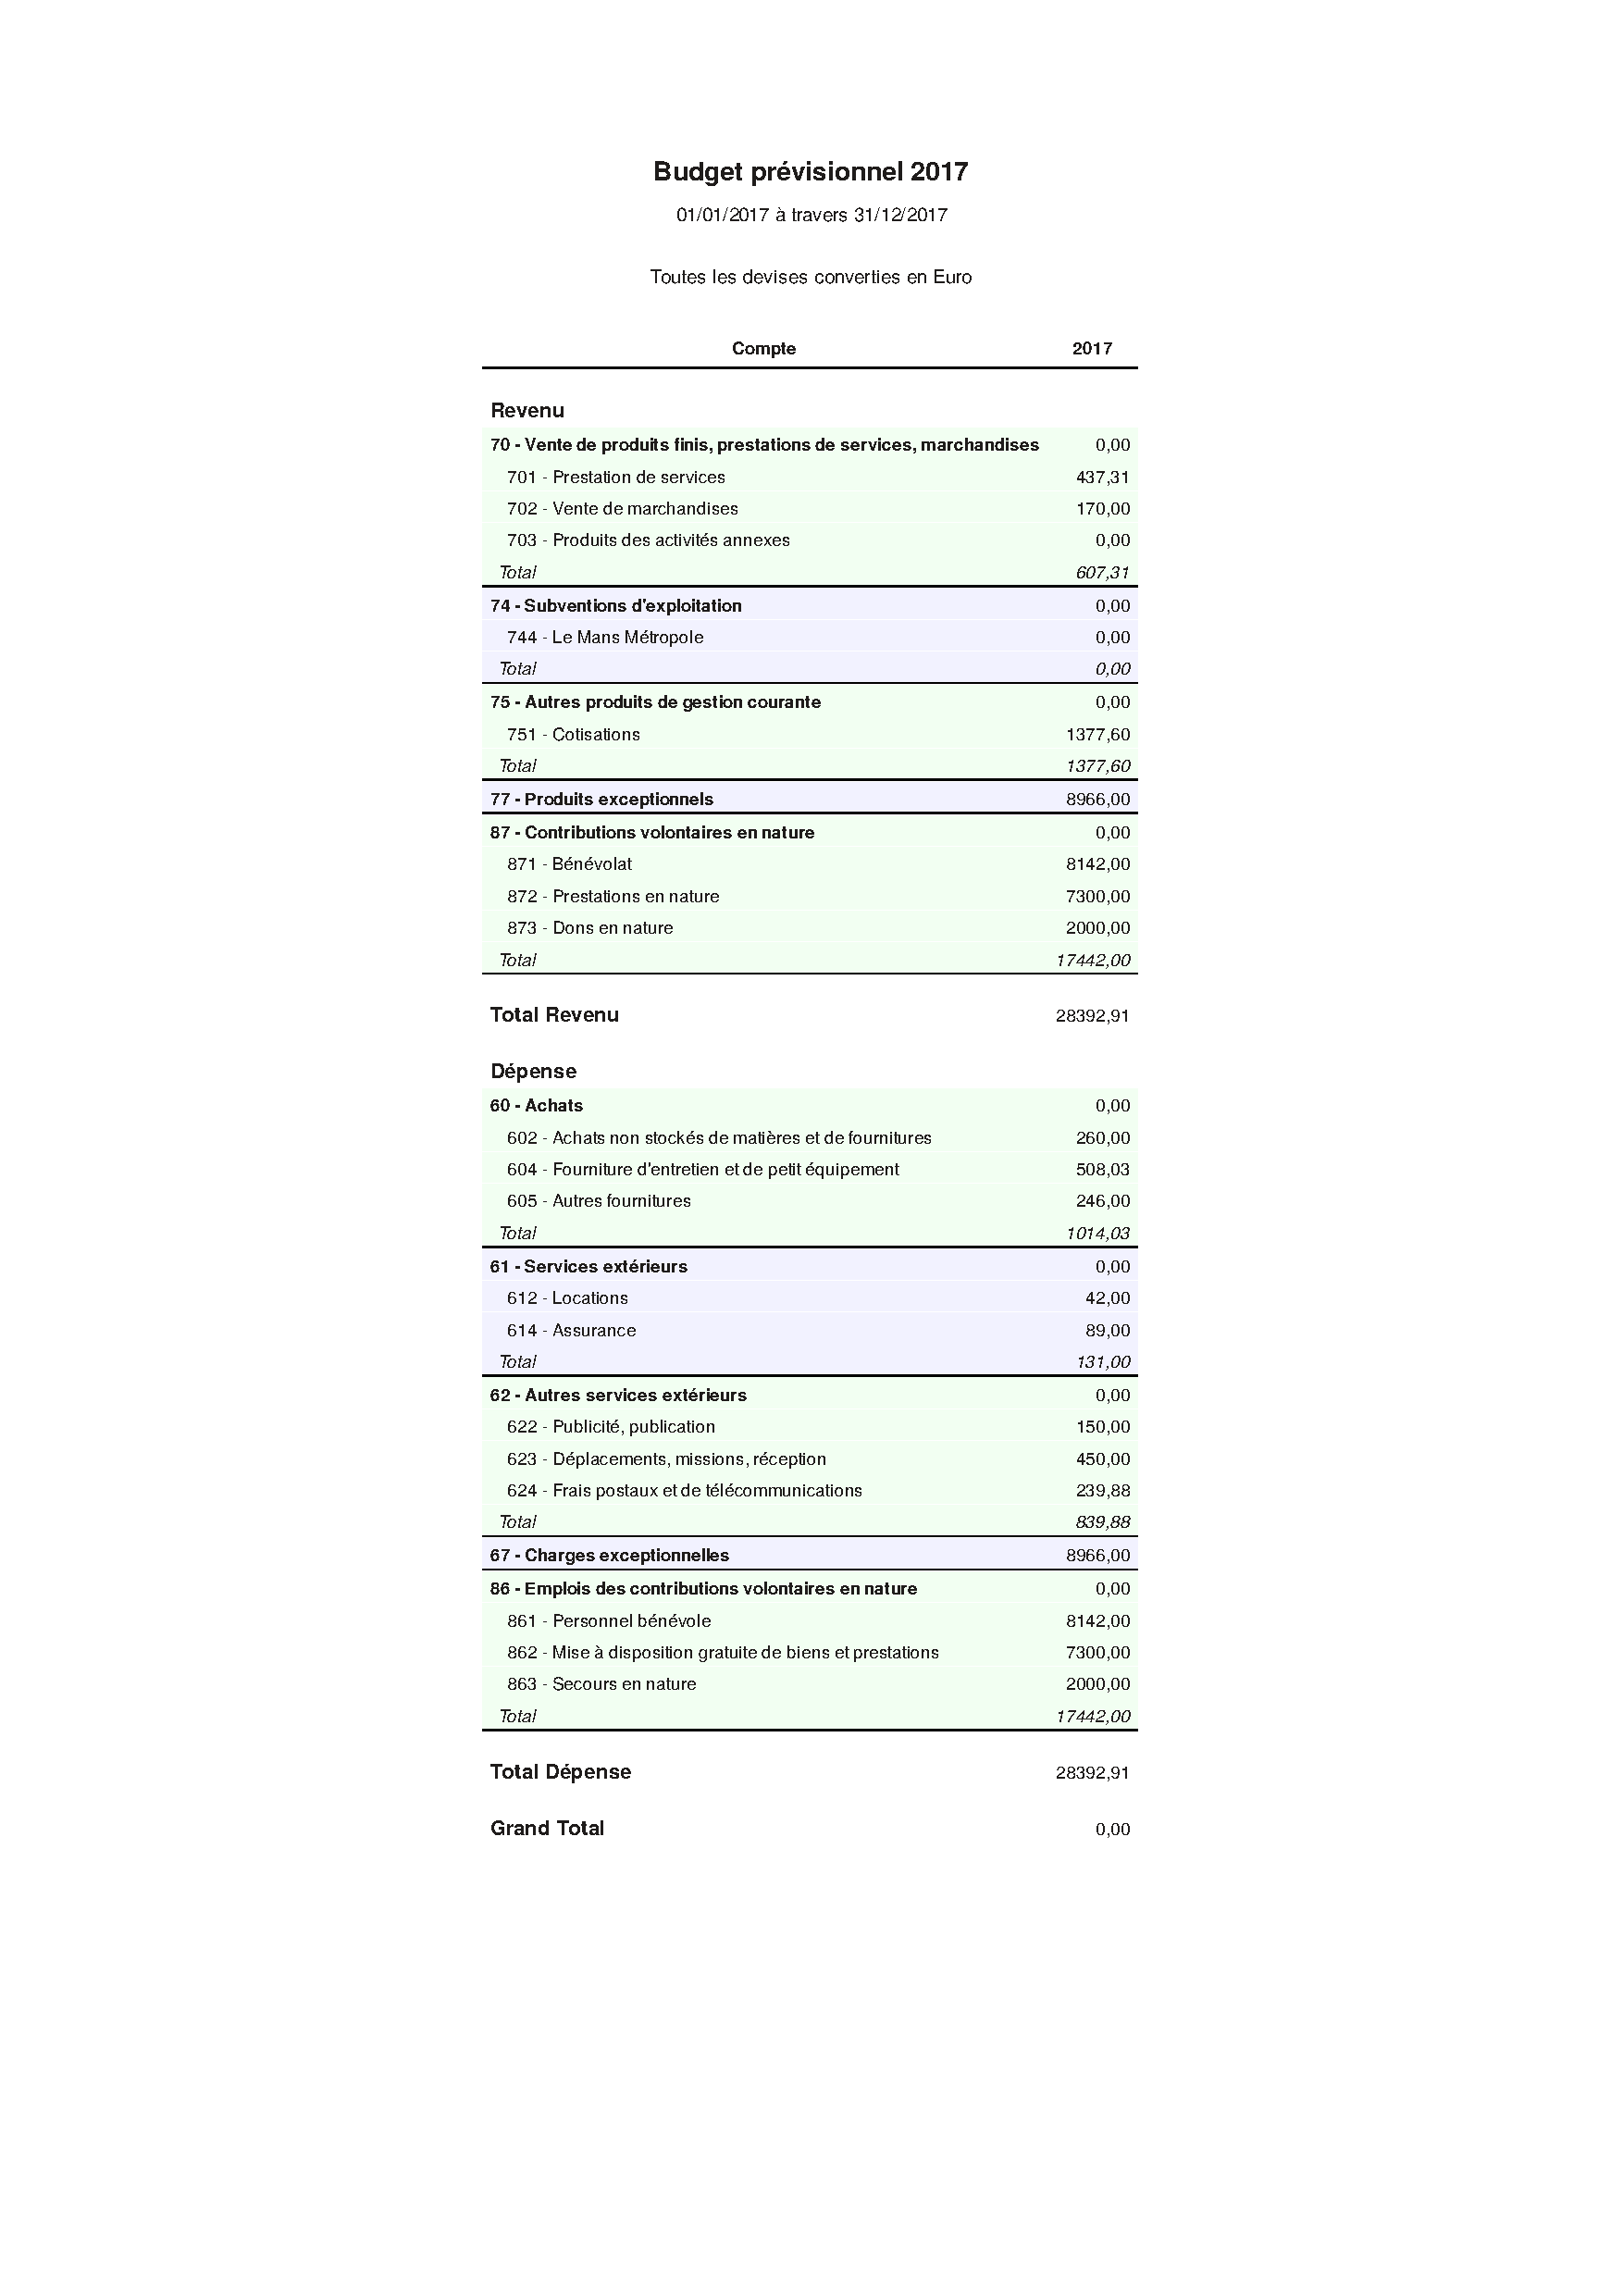
\includepdf[pages=-]{BudgetPrevisionnel2017.pdf}

\end{document}
